\chapter{Introduction}

``Geman quote''

{\em Why pose estimation?}

The idea of an intelligent robot performing a variety of mundane and 
extraordinary tasks, up to and exceeding human performance, has captured the 
hearts and minds of people since at least The Renaissance.  A key feature of 
much of this romantic vision is that robots can interact with {\em us} - 
working with, around and for humans.  An understanding of human pose is a 
crucial component to making this compelling dream becoming a reality.  

In the more practical and not-too-distant future, understanding human pose from 
images has enormous potential to help in many computer vision tasks: semantic 
indexing of images and video~\citep{posesearch}, action 
recognition~\citep{pose-action11}, human-object interaction~\citep{bangpeng12}, 
scene understanding~\citep{gupta11}.   

AI philosopical question - humans can do it, babies,  dogs can do it - why 
can't a computer

Challenging problem: Human pose estimation inherits all the difficulties of 
object recognition - it shows off computation

For all these reasons, the task of estimating a human's pose from visual input 
is a worthwhile and timely problem.  



\section{Problem Statement}

Here we formalize our problem definition input, output and computational 
requirements as follows:  

\begin{problem}[2D human upper-body pose estimation]
\label{prob:pose}
\hspace*{\fill}
\begin{itemize}
 \item[Input:] A single RGB image or RGB video sequence containing the rough 
location and scale of a person in every frame, with no additional information.
\item[Output:] The locations of the major anatomical parts \{left and right 
upper arms, left and right lower arms, torso, head\}.
\item[Requirements:] Computation time and space polynomial in the number of 
input pixels and number of output parts.
\end{itemize}
\end{problem}

\begin{figure}[tb]
\begin{center}
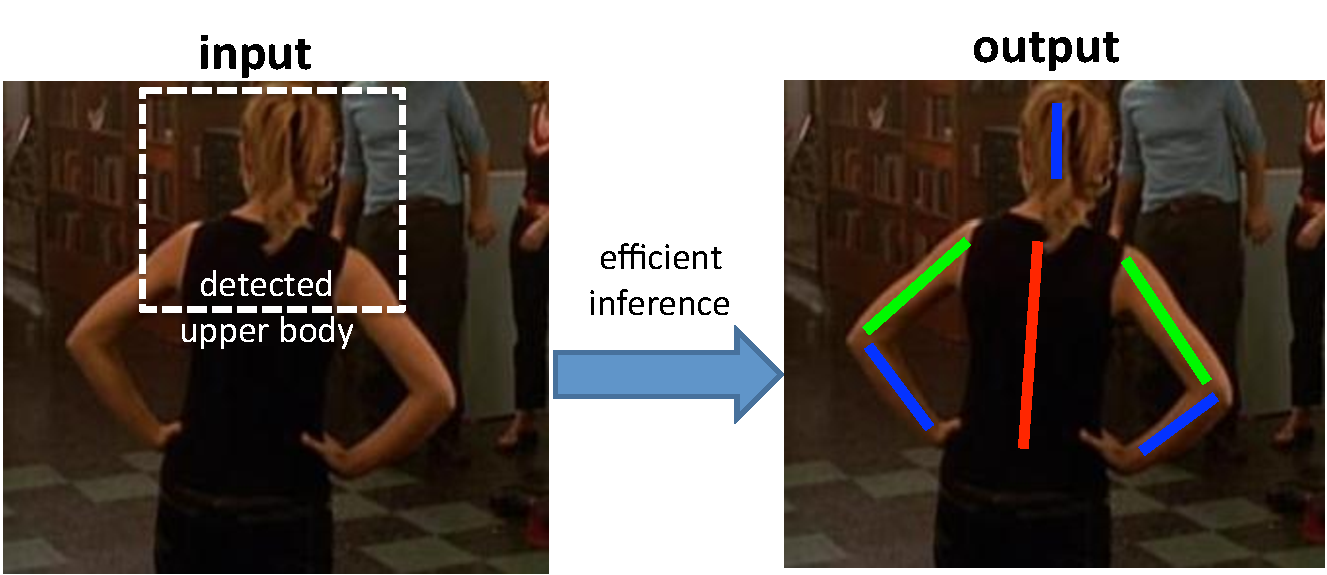
\includegraphics[width=0.95\textwidth]{figs/problem-statement.pdf}
\caption[Statement of problem.]{An example illustrating the pose estimation 
problem, formalized in~\probref{pose}.}
\label{fig:pose-problem}
\end{center}
\end{figure}

Importantly, we concern ourselves only with 2D (two dimensional) input.  This 
makes the task much more challenging than when using additional sensors, such 
as in Microsoft's Kinect capture system~\citep{kinect} where depth information 
and hence reliable knowledge of the background can be used.  However, our 
limited-sensor problem also means it can be applied in more general settings: 
pose estimation outdoors and the wealth of archival images and footages already 
stored on personal computers, libraries, and photo and video sharing web sites.  

Furthermore, we do not assume any additional information, such as knowledge of 
the foreground, background, clothing, lighting, indoor or outdoor, etcetera.  
All these factors work to confound estimation by introducing appearance 
artifacts.  We casually refer to out general setting as pose estimation {\em in 
the wild}, to stress the fact that the data sets we consider feature 
unconstrained foreground and background (or nearly unconstrained, when the 
input is from TV shows).

Also of note, we only consider the upper body, although all methods and models 
discussed in this work can be extended to full body processing (\ie including 
hips and upper and lower legs).  In fact, most of the models and tools develope 
in this work can be applied to other articulated objects, and in general, other 
domains in which estimating the instantiation of interacting parts (\eg, 
handwriting recognition, or gene sequencing). We focus on the upper body human 
pose in this work because (1) most interesting pose variation occurs in the 
upper body, (2) there is a vast amount data of people's upper bodies from TV 
shows, movies and images where lower halves are not visible, and (3) there is 
little extra knowledge to be learned about pose estimation by including the 
lower body parts, while increasing the computation time of all models at least 
linearly.  

Finally, we restrict ourselves to polynomial running time.  The space of all 
possible poses is exponential in the number of parts, and in some sense, the 
ideal thing to do if computation were free is enumerate all possibilities and 
score them holistically.  However, this is simply not feasible, and we are 
forced to make conditional independence assumptions between certain parts to 
achieve tractability.

\section{Intrinsic difficulties}
Human pose estimation in the wild is an extremely challenging problem.  It 
shares all of the difficulties of object detection, such as confounding 
background clutter, lighting, viewpoint, and scale, in addition to
significant difficulties unique to human poses.  We are forced to reason over 
an enormous number of plausible poses for each image, making this a very 
compuationally demanding problem.  In this section we go over the intrinsic 
difficulties of this problem, both from a vision and computational standpoint.

\subsection{Perceptual issues}\label{sec:perceptual}
\begin{figure}[tb]
\begin{center}
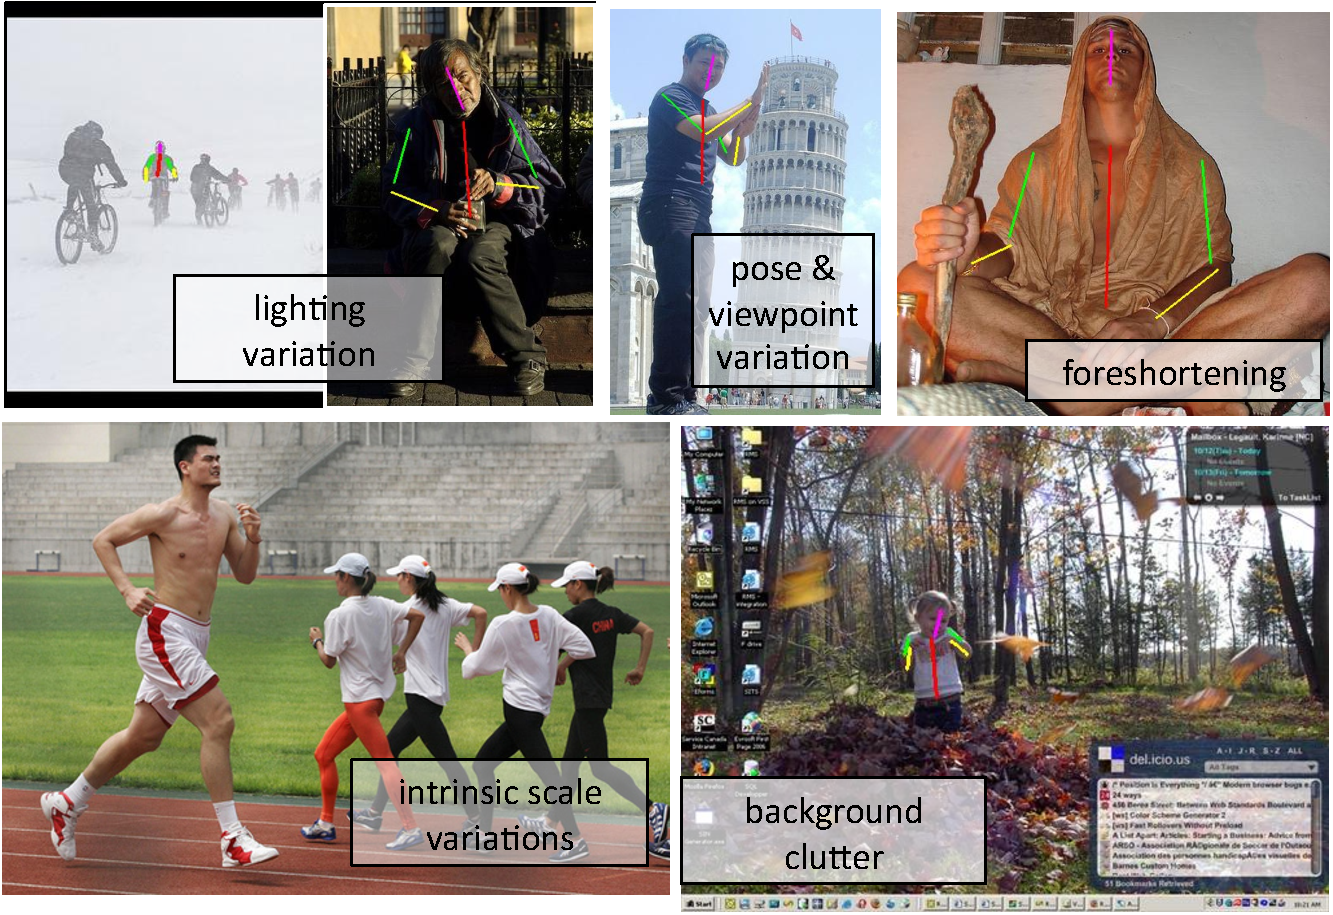
\includegraphics[width=1.05\textwidth]{figs/perceptual-issues.pdf}
\caption[Perceptual difficulties in pose estimation]{Some of the perceptual 
challenges in human pose estimation.  Large variations in lighting, pose, 
viewpoint, foreshortening, relative scale and clutter all work to confound pose 
estimation.  See~\secref{perceptual}}
\label{fig:perceptual-issues}
\end{center}
\end{figure}

This is a difficult problem primarily because the appearance of pose is largely 
unconstrained, making it highly variable with multiple appearance modes.  Some 
issues are as follows, illustrated by~\figref{perceptual-issues}.

\mypar{Lighting:} Images of pose can be taken indoor or outdoor, making not 
only the mean intensity of the image variable (signal bias), but also contrast 
(signal gain). This issue is well studied in computer vision, and to an extent, 
features have been developed to be invariant to lighting, \eg, HoG~\citep{hog}, 
but require harsh quantization and local normalization of edge energy 
information. 

\mypar{Viewpoint and pose: } Humans can look very different depending on the 
angle they are to the camera.  The global ``twist'' (rotation about the 
length-of-body axis) which determines the degree of frontal versus profile 
stance of the person, can be somewhat mitigated by coarse person 
detectors~\citep{andriluka2010}.  However, the body can also go through radical 
appearance changes due to the articulation of the limbs, forcing practical 
systems to decompose the modeling into the most basic, articulation invariant 
components as basic units: limbs and joints.

\mypar{Relative scale:} Although we assume as input a detected person at a 
rough global scale, we have still have a large variation in the scale of parts 
in two different ways: In any particular person, the ratio of limb lengths may 
not be consistent; \eg a baby's proportions versus an adults.  Across people, 
there is also a large differences in the geometries of parts, based on gender, 
body type (fat, skinny, muscular), and age.  These further contribute to the 
variability in appearance.

\mypar{2D projection:} The fact that we are working with images that are 
projections of the real world lead to further difficulties.  Foreshortening 
makes estimating the length of the limb in 2D coordinates even more difficult, 
and changes the appearance.  Self-occlusions and foreground occlusions make a 
part invisible and are very hard to determine without further scene or depth 
knowledge.  Finally, it is inherently ambiguous to map from 2D pose to 3D real 
world coordinates (even up to an unknown global scale factor), discussed 
further in~\secref{limitations}.  This makes it difficult to model priors on 
arm length, as we are forced to measure and reason about lengths on the 2D 
pixel grid.

\mypar{Clothing:} There is potential for even more variation in clothed people 
than there is in the space of naked bodies.  Not only is clothing responsible 
for foreground clutter, it also can be considered an occluder which hides parts 
(\eg baggy clothing, skirts, ponchos) and can break assumptions about 
left-right appearance symmetry (\eg an asymmetric shirt).

\mypar{Background clutter:} \todo{forgot this one}

\begin{figure}[tb]
\begin{center}
\includegraphics[width=1.05\textwidth]{figs/dataset-multimodal.pdf}
\caption[Variations in appearance]{Some illustrations of variation in 
appearance in the PASCAL Stickmen dataset.  (a) An average of the dataset in 
grayscale.  (b) Average of sobel edges over dataset.  (c) Distribution of inner 
angle made between upper and lower arm, with examples for 
$0^\circ,45^\circ,90^\circ,135^\circ,180^\circ,225^\circ,270^\circ$ and 
$315^\circ$. (d) A random sampling of 100 left elbows from the Buffy Stickmen 
pose dataset,	removing color and intensity bias, to illustrate the huge variety 
of appearance due to	clutter, motion blur, clothing, body type, and pose.  
\label{fig:dataset-multimodal}}
\end{center}
\end{figure}



\subsection{Computational issues}

To operationalize ~\probref{pose}, let $x$ be the input image pixels, and $y$ 
be a representation of the output predicted pose.  Then a general solution 
to~\probref{pose} would take the form of a {\em scoring function} $h(x,y)$ 
which evaluates the quality of any estimated pose $y$ in the image $x$.  We can 
define the ``best'' pose as the highest scoring: $y^\star = \argmax_y h(x,y)$ 
(or $y^\star = \arg\sup_y h(x,y)$ if $y$ is infinite dimensional, \eg 
continuous).  Then~\probref{pose} is satisfied if this determination of the 
maximizer can be done in polynomial time. There are two sources of intrinsic 
computational complexity within this framework. 

\mypar{Complexity of the input:} For the reasons outlined 
in~\secref{perceptual}, there are an astronomical number of different inputs 
$x$ that can map to the same true pose $y$, due to changes in the background, 
foreground, scene properties, camera effects, and variations in human pose, 
bodies and clothing.  This makes modeling the space of poses from the input 
extremely difficult.  The problem is inherently multi-modal, in the sense that 
radically different appearances are equally valid input representations of any 
particular pose.  For a few different illustrations of the variability of a 
dataset, see~\figref{dataset-multimodal}. 

To deal with this complex problem, we are forced to either design features that 
are invariant to the multi-modal nature of the problem (\eg, a generic 
patch-based arm detector based on coarse edges, or geometric features based on 
relative part coordinate systems), or to partition the space and model multiple 
modes separately.  In the case of the latter approach, we are faced with other 
difficult decisions regarding model complexity: how to define modes and a 
notion of locality, and what the right trade-off is between the richness of the 
model and the error in fitting the model at different modes with a finite 
amount of training data.

\mypar{Complexity of the output:}
The enormous combinatorial space of possible output poses is a second source of 
computational complexity.  A typical discretization of the state space of human 
poses is an $80 \times 80$ spatial grid of part locations at $24$ possible 
angles~\citep{felz05}, resulting in an output space that is roughly $150000$ 
possibilities for each part, and thus $150000^6 \approx 10^{30}$ for the joint 
output space of all $6$ parts~\footnote{In the case of continuous spaces, the 
output space is infinite (infinitely precise), and to maintain tractability the 
form of $h(x,y)$ is typically analytical with a closed-form maximum, mean 
and/or mode.}.

Enumerating all possibilities for a joint configuration of all parts is clearly 
not feasible.  At the other extreme, we could ignore part interactions, and 
estimate the pose of each part separately---a task which instead has $6 \times 
150000$ possibilities, which is very computationally cheap.  However, 
individual part detection is extremely difficult for body 
parts~\citep{andriluka09} due to the wide range of appearance and lack of 
discriminating features.

Between the two extremes of (1) estimating parts in isolation and (2) 
enumerating all possible joint pose configurations, there lies a family of 
models $h(x,y)$ that consider {\em some} part interactions, but not all.  The 
simplest of these is a {\em first-order} model which looks at pairs of part 
interactions at a time, and the graph of part interactions forms a tree 
structure.  This compromise between a full model of every part and a decoupled 
model of independent parts will be the basic model building block throughout 
this work.

In such a first-order, or {\em pairwise} model, the basic bottleneck operation 
is to evaluate the quality of a pair of parts at a time. The model combines all 
such pairwise scores together to determine the optimal global pose.  This 
scoring requires $150000^2 \approx 1$ billion possibilities to consider, which 
is large but just small enough for modern machines to handle with some 
additional model restrictions, detailed in~\secref{ps}.

\todo{reduce from NP-hard problem?}

\section{Contributions of this thesis}

Due to the computational issues discussed above, previous work in pose 
estimation has resorted to a model of pose that considers, at most, pairwise 
interactions between parts, in a specially restricted form:
$$ h(x,y) =  \sum_{i \in \cV_{\tree}} \phi_i(x,y_i) + \sum_{i,j \in 
\cE_{\tree}} \phi_{ij}(y_i - y_j) $$
where the network of part pairwise interactions is described by a tree 
structured graph $\tree = (\cV_\tree,\cE_\tree)$.  The first terms 
$\phi_i(x,y_i)$ how likely a part is to be placed at location $y_i$, 
independent of other parts.  The pairwise term $\phi_{ij}(y_i-y_j)$ simply 
measures the geometric compatibility between pairs of parts.  Importantly, this 
pairwise term is {\em blind to the image content}.  As we will see 
in~\secref{ps}, this simple form has been historically necessary in order to 
find the highest scoring global pose quickly.

Such a simplistic pairwise would be admissible if the individual part terms 
were sufficiently accurate on their own.  However, for reasons discussed 
in~\secref{perceptual}, individual part detector scores are extremely weak: 
they must work in isolation and generalize to limbs in all settings of 
backgrounds, foregrounds, articulation, and environment.

As a result, the above model is effectively trying to piece together parts of a 
person, when the parts themselves are extremely ambiguous. As an extreme 
analogy of this, it is like attempting to put together a jigsaw puzzle in which 
the pieces themselves are very generic, and to determine whether two pieces fit 
together, you can only observe their boundary geometry, and {\em not } the  
image content on their faces.


\subsection{Image-dependent interactions via a cascade of models}
Instead, we wish to actually {\em exploit } image content when modeling 
pairwise interactions.  In the puzzle analogy, this would allow us to fit 
pieces together based on their color similarity and continuous contours across 
the connection boundary.  We exploit these same cues for determining whether 
limbs go together in an image, as well as additional cues such as region 
support and multi-modal descriptions of geometry.

To this effect, we propose a more general model of human pose, of the form 
\begin{equation}
h(x,y) =  \sum_{i \in \cV_{\tree}} \phi_i(x,y_i) + \sum_{i,j \in \cE_{\tree}} 
\phi_{ij}(x,y_i,y_j)
\label{eq:contrib1}
\end{equation}
This turns out to be computational infeasible using standard tools and techniques.  In light of this, we propose a {\em cascade} of models to focus computation on portions of the state space that are more promising.  The key insight is that there are many pose possibilities that are easy to reject as incorrect with a simple model, and we are then able to freely apply a richer model on the possibilities that remain.  This is illustrated in~\figref{cps-overview}.

We develop and analyze {\em structured prediction cascades}, and apply them to the problem of 2D pose estimation, allowing us to use a model in the form of~\equref{contrib1} at every level of the cascade.  Importantly, we provide a novel learning objective for the cascade of models so that parameters of the model are tuned to specifically to filter out a a significant proportion of states at any intermediate level. 


$$ \max_y \sum_{i \in \cV_{G}} \phi_i(x,y_i) + \sum_{i,j\in  \cE_{G}} \phi_{ij}(x,y_i,y_j) $$
$$ \max_y \max_z \sum_{i \in \cV_{G}} \phi_i(x,y_i,z) + \sum_{i,j \in \cE_{G}} \phi_{ij}(x,y_i,y_j,z)$$

